\documentclass[a4paper,12pt]{article}
\usepackage{ecography}
\usepackage{lmodern}
\usepackage{amsmath}
\usepackage{xfrac}

 \renewcommand{\familydefault}{\sfdefault}


\title{A Recipe for Scavenging - the natural history of a behaviour}
%TG: nice title! I'd replace the hyphen with a comma though
\running{Scavenging in vertebrates}

\author{Adam Kane, Kevin Healy, Thomas Guillerme, Graeme Ruxton, \& Andrew Jackson.}

\affiliations{
\item A. Kane (\url{adam.kane@ucc.ie}), University College Cork, Cooperage Building, School of Biological Earth and Environmental Sciences, Cork, Ireland.
\item K. Healy and A. Jackson, Trinity College Dublin, Department of Zoology, School of Natural Sciences, Dublin Ireland.
\item T. Guillerme, Imperial College London, Silwood Park Campus, Department of Life Sciences, Buckhurst Road, Ascot SL5 7PY, United Kingdom.
\item G. Ruxton, School of Biology, Sir Harold Mitchell Building, Greenside Place, St Andrews, KY16 9TH, United Kingdom.
}

\nwords{9999}


\begin{document}

 \maketitle


\begin{abstract} 
% Here, we chart the natural history of scavenging. 
Despite its prevalence, scavenging is a difficult behaviour to observe in modern day carnivores and impossible to study directly in extinct species. 
Yet, there are certain intrinsic and environmental features of a species that push it towards a scavenging lifestyle. 
These can be thought of as some of the principal parameters in optimal foraging theory namely, encounter rate, handling time and prey availability. 
% Chief among these are low-cost locomotion, high detection distances, effective carcass processing and a carrion-producing habitat. 
We use these components to highlight the morphologies and environments that would have been conducive to scavenging over geological time by focusing on the dominant vertebrate groups of the land, sea and air. 
The result is a document on the natural history of scavenging, the first to our knowledge. 
Our idea of a scale of scavenging can be applied to any species at any time to judge the importance of this behaviour in its diet. 
\end{abstract}

\newpage


\section*{Introduction}

Historically, scavengers have not been viewed as the most charismatic of animals.
This may go some way to explaining the gap in our knowledge of the prevalence of this behaviour \citep{devault2003scavenging}.
Professor Sanborn Tenney writing in 1877 for The American Naturalist had this to say about one well known group, ``prominent among the mammalian scavengers are the hyenas, the ugliest in their general appearance of all the flesh eaters."
He contrasts these with ``nobler kinds" of carnivores such as lions and tigers \citep{tenney1877few}.
Even aside from our own subjective biases, scavenging is a difficult behaviour to detect after the fact.
Without catching a carnivore in the act of killing we are left to infer how the prey was killed.
Some simple heuristics can inform us, for instance, in cases where the prey item was simply too large to have been killed by the ostensible predator \citep{pobiner2008paleoecological}.
But clearly, a scavenger doesn't only feed on animals too big for it to have hunted.
The obvious lack of direct behavioural data compounds the difficulty of discerning scavenging among extinct forms.
Indeed, a single species of dinosaur notwithstanding \citep{carbone2011intra}, a synthesis describing the natural history of scavengers is absent from the literature.
%TG: I don't understand the dinosaur part of this sentence. Might be my non-native english but I thought it's worth noting for other non-english folk out there (even though I know they aren't many!).
Fortunately, research on scavenging is on the rise \citep{manga2006vulture}.
As a result, we are now beginning to realise the extent of this behaviour such that, ``in some ecosystems, vertebrates have been documented to assimilate as much as 90\% of the available carrion" \citep{beasley2015vertebrates}.
This has profound implications for the trophic ecology of these systems and particularly our models of them.
Even Tenney’s noble big cats are now known to take in a significant portion of carrion in their diet where some lion populations get over 50\% of their meat from carcasses \citep{jones2015african}.
By recognising the difficulty in directly observing scavenging, other methods have been turned to to discern the most suitable morphologies, physiologies and environments for a scavenging lifestyle to prosper.
Here we chart the natural history of scavenging by assessing the potential for the behaviour in dominant vertebrate groups given their ecology and functional traits.
%It is our aim in this review to employ these methods to gain an understanding of scavengers past and present.

%the intro needs to lead towards a aim a bit more strongly

\subsection*{The Challenges of Scavenging} %TG: challenges or difficulty? up to you.
The chief hurdle to scavenging is finding a resource that is often difficult to predict in space and time.
Through chance alone many species will avail of some opportunistic scavenging. %TG: Two times "opportunities", replaced by "chances"
However, species that rely on scavenging to sustain substantial portions of their diets must increase the probability of encountering a sufficient amount of carrion in order to meet their energetic demands.
%Once found, the scavenger must be able to out-compete any potential competitors and process a product under the processes of decay from toxin producing and disease causing microorganisms \citep{ruxton2014fruit}. %TG: make the following sentence more sense?
Once found, the scavenger must be able to out-compete any potential  competitors and process the, typically decaying, carcass replete with microorganism derived toxins  \citep{ruxton2014fruit}.
Finally, the potential for scavenging will also depend on the density, size, and quality of carcases produced, all of which are affected by complex ecosystem dynamics.
All of these facets are essentially the key parameters found in functional response curves, namely encounter rate, handling time and prey availability \citep{jeschke2002predator}. %TG: Jaysus, this sentence doesn't read well! "Functional response curves of optimal foraging theory" can probably be phrased in a nicer/easier way...
%With this framework we compare the ability of scavenging across vertebrates. % focusing on each of these facets and their relationship with scavenging.
By considering scavenging in this context of optimal foraging we can identify the prerequisite attributes and processes required for the behaviour. 
This has enabled us to propose a scale of scavenging whereupon we can place any vertebrate species, past or present, and assess the importance of carrion in its diet. 

\begin{figure}[!htbp]
\centering
   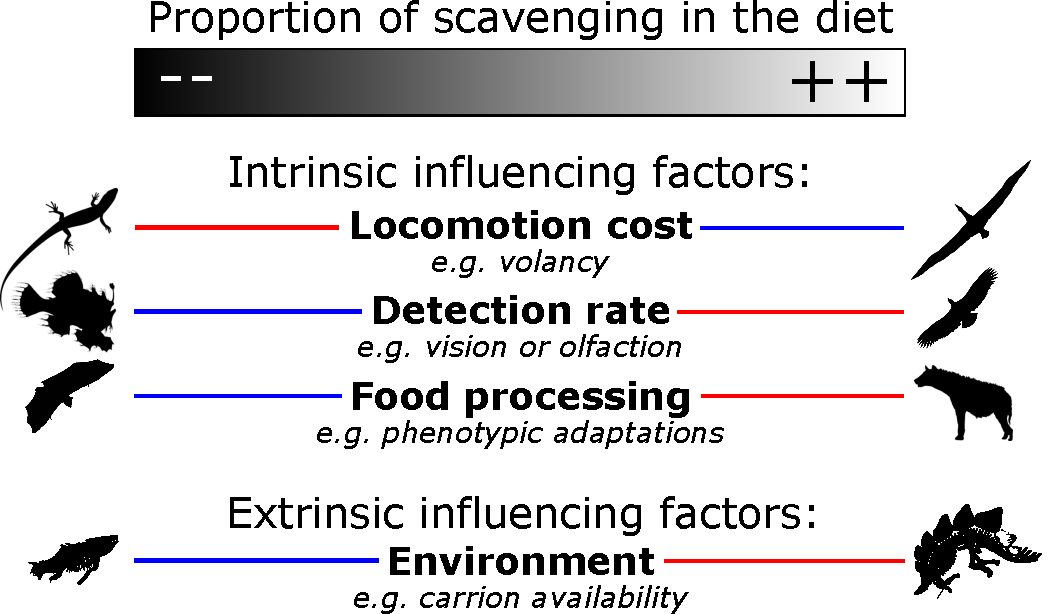
\includegraphics[width=1\textwidth]{Summary_figure/Summary_figure_Landscape.pdf}
\caption{Factors influencing the proportion of scavenging in a vertebrates' diet. Blue lines indicate a reduction in the factor and red lines indicate an increase.}
%TG: Probably needs some more explanations...
\label{Summary_figure}
\end{figure}

%KH: need paragraph for how do we know something is (was) a scavenger
\section*{Encounter Rate}
All foraging processes depend on the encounter rate between consumer and resource. 
In the simplest case, this rate can be thought of in terms of a gas diffusion model where the movement of two agents (i.e. predator and prey) depends only on their relative speed.
Vertebrates do more than simply bump into resources like gas molecules though, because predators can actively detect prey through their sensory abilities. %TG: I like the gas diffusion analogy but it might be adding too much text and be not essential. I've added some precisions though.
As carcasses are stationary, the relative speed between a scavenger and carrion is only dependent on the movement of the scavenger.
As such, scavenging potential is strongly affected by search rates, which are determined by both species' physiology and the dimensionality of the environment \citep{pawar2012dimensionality}.

\subsection*{Locomotion}
Because of the inherent unpredictability of carrion, scavenging depends more on the ability to efficiently move over large areas than predation.
This generally requires an efficient transfer of metabolic energy into movement which relies on both physiology (i.e. metabolism) and the medium of the environment in which the animal is moving (i.e. aerial, aquatic or terrestrial).
Perhaps the most efficient form of locomotion in vertebrates is, paradoxically, found in flying species. 
Despite the energetic costs of flight, the only known vertebrate obligate scavengers are the old and the new world vultures. 
And, although powered flight is energetically expensive, species like vultures can exploit air currents using their large wingspans which allows them to soar at a cost of only twice their metabolic rate \citep{hedenstrom1993migration,spivey2014analysing}.
By depending on thermal air flows these species can forage over vast ranges \citep{spiegel2013factors}. 
An analogous mode of locomotion is also exploited by seabirds, who use strong ocean winds to search large areas of the oceans \citep{norberg2012vertebrate,thaxter2012seabird}. 
While many species of seabird are likely primarily predators, it seems that albatrosses, who can range many hundreds of kilometres, take a substantial amount of carrion in their diet \citep{croxall1994dead}. 
This is typically in the form of squid carcases, which float on the surface, allowing the birds to readily pluck their remains out of the water \citep{croxall1994dead}. 

The groups from which modern vultures and seabirds arose, appear during the Palaeocene \citep[66 - 56 Million years ago (Mya); ][]{Jetz2012, Jarvis2014} and Cretaceous \citep{chiappe2006early} respectively.  % KH and are likley to have being soaring fliers as demonstrated by their large wingspans (Is this true?). (Is there any other form of soaring?).  AK I don't think this is true from what I've seen
However, soaring flight is likely to be far older than this with avian flight originating in the Late Jurassic (163.5-145 Mya) and vertebrate flight in the Late Triassic (235-201.3 Mya) coincident with the pterosaurs. 
Indeed, scavenging among pterosaurs has been hypothesised many times before \citep{witton2008reappraisal}. 
Certain groups of these animals could reach enormous sizes \citep[e.g. Azhdarchids with wingspans of 11 metres; ][]{witton2010size} and, notably, appear to have engaged in soaring flight \citep{witton2010size}.
It seems probable that extinct species used soaring as a means for scavenging \citep{witton2013pterosaurs}. 

While soaring is perhaps the only viable means of locomotion that allows for an obligate, scavenging life-style \citep{ruxton2004obligate}, powered flight is still an efficient means of locomotion. 
Certainly, avian flight is cheaper than either walking or running \citep{tucker1975energetic}.
%TG: I'd rather put the following part as an appendix or foot note. Reader can take our (Tucker's) word for it and then check the math to see that even with maintenance and blablabla flying wins.
%Even taking account of maintenance costs, this still bears out, where total cost of movement (J kg\textsuperscript{-1} m\textsuperscript{-1}) scales according to 5.2 $\times$ body mass (kg) \textsuperscript{-0.23} for fliers and 10.7 $\times$ body mass (kg) \textsuperscript{-0.32} for runners \citep{williams1999evolution}.  
%TG: This also allows to link directly to the next argument in the same paragraph: facultative active flying scavengers.
We know that many extant birds exist as facultative scavengers because storks, raptors and corvids all take substantial quantities of carrion in their diet \citep{kendall2013alternative}. 
Similarly we would expect that extinct species would also scavenge in a similar fashion depending on the efficiency of their flight. 
For example, early birds such as \textit{Archaeopteryx} are predicted to have been poor, relatively inefficient fliers \citep{nudds2010narrow} and so ill-suited to finding carrion. 
%Similarly something about the efficiency of pterosaurs flight. TG: Was this a comment? By the way, about pterosaurs (though it might not be necessary to mention it), most of them where tiny little feckers like Archaeopteryx or even smaller.

The importance of efficient flying over large areas may explain the lack of scavenging behaviour in bats as they are generally nocturnal, a time when they would receive no aid from convective air currents \citep{norberg2012vertebrate}. 
%smaller and less efficient in comparison to larger birds (speculating here but I wouldnt be surprised), %AK Don't think it is the case that bats are less efficient than birds in terms of flight 
That said, \textit{Necromantis} (``death-eater''), a large bat from the middle to late Eocene (56-33.9 Mya) had a robust cranio-mandibular morphology, and is a likely candidate for scavenging behaviour \citep{Weithofer_Necromantis_1887,Hand_Necromantis_2012}.% amongst the x amount of known bat species \citep{Weithofer_Necromantis_1887,Hand_Necromantis_2012}. %TG: we can cut this number of bat species to avoid getting into stamp collecting debate. + there are effectively a two shit load units of them which makes the Necromantis example not really convincing.

Similar to aerial species, aquatic scavengers have a locomotory benefit because water is a medium that is conducive to low-cost movement \citep{tucker1975energetic,williams1999evolution}.
%TG: Same as comment before, maybe put the following as a footnote or as a supplementary.
% In fact, the total cost of movement (again in J kg\textsuperscript{-1} m\textsuperscript{-1}) in salmonids is lower than either running or flying where it scales according to 2.15 $\times$ body mass (kg) \textsuperscript{-0.25} \citep{williams1999evolution} with only \textit{soaring} flight likely to surpass it. 
%KH(I assume the reference is for powered flight, again this needs to be more precise).  
This has led some researchers to argue for the likelihood of an obligate scavenging fish \citep{ruxton2004energetic,ruxton2005searching}. 
Interestingly, style of swimming in fish does not significantly affect the cost of movement \citep{williams1999evolution}. 
Though sharks perhaps best resemble the large soaring fliers as they depend on large pectoral fins in order to maintain lift as they swim. 
Many shark species have large foraging ranges \citep[e.g. the great white sharks \textit{Carcharodon carcharias};][]{bruce2006movements} and it seems reasonable that they would use oceangraphic currents to further reduce movement costs \citep{ruxton2004energetic}. %and are able to maintain a type of endothermy from thier movements \citep{bernal2015sharks}. %TG: I guess the following is a comment: (I know the Greenland shark is the slowest swimmer). 
In fact, facultative scavenging is seen in many selachian groups, including species of extant sharks like white sharks \citep[known to feed on whale carcasses;][]{fallows2013white}, Greenland sharks \citep[feeding on seals;][]{watanabe2012slowest}, and sixgill sharks \citep{anderson2016impact}. 
The former which grow up to 6 metres long, can be sustained by 30 kg of whale blubber for over six weeks \citep{carey1982temperature}. 
There is evidence too of scavenging in extinct species, where shark teeth have been found in the remains of dinosaurs, mosasaurs and Pliocene mysticete whales \citep[5.3-3.6 Mya; ][]{schwimmer1997scavenging,ehret2009caught}. 

% KH Other types of swimming in fish, other species propelled by fins (turtles and plesiosaurs etc)

% KH snakes - ie undulating

% KH endotermy - why it doesn't seem to work
We might expect then that by combining an aquatic environment and an endothermic metabolism marine mammals would especially prosper as scavengers.
Fossil pinnipeds and cetaceans from 60 Mya %TG: that early???
have transitional features indicative of their trajectory to fully aquatic species \citep{williams1999evolution}.  
But despite their movement away from land their energetic savings were negligible because the \textit{total} cost incurred by a swimming marine mammal is high \citep{williams1999evolution}. 
Indeed, the total energetic cost is similar to an equivalent terrestrial or aerial mammal \citep{williams1999evolution}.
This underscores the trade offs between the benefits of endothermy in terms of activity periods and the costs of maintaining such an expensive system. 
That said, aquatic endotherms have and do scavenge. 
For instance, early whales such as \textit{Basilosaurus} (38-36.5 Mya) seem to have fit into the same niche as killer whales (\textit{Orcinus orca}) and we have some evidence for scavenging in both \citep{fahlke2012bite,Whitehead415}.
%\cite{williams1999evolution} notes, ``free-ranging animals must contend with the total energetic expenditure associated with supporting basic biological functions as well as with moving the body and appendages through the environment."

%% AK:  Need to be careful here because this whole idea of sprawling posture being worse off than erect posture is not that well supported in the literature. 
%% Great Transformations in Vertebrate Evolution By Kenneth P. Dial, Neil Shubin, Elizabeth L. Brainerd talks about it at length 
%% So I think this should stay pitched as an endo/ ectothermy thing rather than posture 
Terrestrial environments are the most energetically costly in which to move, which may be due to the low muscular efficiency of running \citep{tucker1975energetic} as well as the relative inefficiency of gas exchange in the case of terrestrial mammals \citep[cf. birds and fish ][]{williams1999evolution}. %TG: Hmm I get the point of gas exchange efficiency but (1) it should be more developed if left like that (i.e. what the flip is meant by gas efficient exchanges) and (2) that works for mammals, but in terms of terrestrial that ignores birds, squamates, crocodiles and amphibians.
%
%TG: It's missing a transition here, we go from gas exchanges to posture. Maybe we need something like "Among terrestrial scavengers, most are mammals. This might be due to the posture blablabalba." But then it doesn't connect logically with the sentence before: "mammals have are inefficient...". Maybe one way is to just remove the gas exchange and start with something like:
%Terrestrial environments are the most energetically costly in which to move, which may be due to the low muscular efficiency of running \citep{tucker1975energetic}.
%Most terrestrial species that have been observed (or are suspected to be) scavenging are mammals.
%TG: and then link to the posture hypothesis (with the "meh, we're not sure" at the end).
%
However, the evolutionary transition in posture from the sprawling gait of reptiles to the erect posture of mammals has often been supposed as conferring a huge advantage to the latter.
The purported advantages include benefits in terms of speed, efficiency, muscle effort and manoeuvrability \citep{sullivan2015posture}. 
Despite being intuitive, \cite{sullivan2015posture} states most of the hypotheses in favour of this idea remain to be tested in the context of archosaur evolution. 
Metabolic rate however, unquestionably impacts terrestrial species whereby ectotherms such as many modern reptiles, cannot move for sustained periods \citep{bennett1979endothermy}. 
% Species which do not support an upright position such as modern reptiles limit their ability to move for sustained periods \citep{bennett1979endothermy}. 
This is exacerbated by their sprawling gait which results in the phenomenon known as Carrier's constraint such that the animal can't move and breathe at the same time because the lateral movements impedes its lungs \citep{carrier1987evolution}. 
% These constraints are likely to mean that many ectotermic terrestrial species, which cannot maintain an upright posture would depend on a relatively low level of scavenging (I'm not sure this is true though). 
This would also have been true of extinct species with the same physiology. 
%TG: I guess this is a comment too: Snakes are a bit different are more effecent at moving I think - lots of scavanging. 
%Both these groups are more likely to depend on low energetic costs in order to compensate for low encounter rates due to their inability to move. 
It is with the evolution of endothermy in the therapsid-mammal lineage \citep{clarke2010temperature} that terrestrial vertebrates would have gained the ability to range more widely, a vital component in seeking out carrion. 
Although the earliest evidence of vertebrate scavenging comes from the Permian (298.9 - 252.17 Mya) where a temnospondyl amphibian fed on the carcass of \textit{Varanops}, a predatory synapsid of the time \citep{reisz2006articulated}. 
%TG: I do like the way all our paragraphs end up with a "But wait, there's an exception!"


Modern endothermic mammals can sustain longer periods of energetically expensive activity \citep{bennett1979endothermy} resulting in larger foraging ranges. 
%TG: Same comment as for the other math, I'd rather put that as a footnote or in the appendix (the whole yoke). Again, it seems a bit disproportionate that for some example, we just dumb a line (or even an example in brackets) and that for some others, we explain the example in details.
% To quantify this effect with a simple example we can turn to some allometric relationships relating sustainable travelling speed to body mass \citep{ruxton2004obligate}.
% If we insert these into a foraging radius model \citep{Enstipp2006Energetics} for a 12 hour foraging day it shows that while a 10 kg reptile can range 6.5 km, an equally sized mammal can range nearly 33 km (See appendix). 
% For a foraging scavenger, this ability translates into a greater area searched for food.
Today, terrestrial scavenging in the mammals is probably best known in an African context where hyenas, jackals and lions all take sizeable proportions of carrion in their diet.
In the spotted hyena (\textit{Crocuta crocuta}), striped hyena (\textit{Hyaena hyaena}) and brown hyena (\textit{Hyaena brunnea}) it can be over 90\% \citep{jones2015african}.
And although no contemporary terrestrial vertebrate exists as an obligate scavenger, most, if not all, are facultative to some extent \citep{beasley2015vertebrates}.
The particular reliance of hyenas on carrion means we can use them as examples of efficient terrestrial scavengers to compare with other forms. 
In terms of locomotion, they employ a characteristic ``rocking horse gait"  which allows them to cover great distances efficiently, loping at 10 km/hr \citep{mills1989comparative,jones2015african}. 
Such long-distance travel is apparent in African wild dogs (\textit{Lycaon pictus}) and many other canids \citep{pennycuick1995radius,janis2014forelimb}. 
In contrast, big cats like leopards (\textit{Panthera pardus}) rely on ambush \citep{pennycuick1995radius}. 
This allows us to make a broad distinction between the ambush strategies of cats-like forms and the pursuit/ pounce strategies of more dog-like forms%TG: I've added the "-like" to underline that we're not talking about the phylogeny here (i.e. not Felidae (incl. hyena) vs Canidae)
, the latter being more suited to scavenging \citep{janis2014forelimb}. 
These insights allow us to compare extant terrestrial species to their prehistoric forebears given the dominance of mammalian carnviores since the Eocene (56-33.9 Mya) where the order split into the Caniforma and Feliforma \citep{van1987skeletal}.
To take one example, \cite{anyonge1996locomotor} found that \textit{Nimravides}, a genus of sabretooth cat from the Miocence (10.3 to 5.3 Mya), were likely to have been ambush predators which would argue against them taking a lot of carrion. 
%The order Carnivora saw its origins in the Middle Eocene  %TG: a phylo side note: the correct sentence would be the "The stem Carnivora saw its origins ... when it split into Caniforma and Feliforma." But I think we can leave it out because, god, it sounds pedantic!
% So we can trace efficient terrestrial movement by carnivores from this point on. 

Of course, terrestrial animals can also move bipedally. 
%TG: missing some transition here. Maybe something short like "Further back in time" or "Previous to that"...
Although the evolution of bipedal movement was significant in that it freed up the forelimbs for other purposes (e.g. climbing, tool-use, wing development etc.) it does not differ radically in cost from quadrupedal locomotion \citep[][and references therein]{williams1999evolution}. 
For instance, \cite{alexander2004bipedal} shows that, in the case of humans, we are more economical than predicted while walking and less so while running according to predicted costs of terrestrial movement. 

Aside from humans and our allies, the best-known terrestrial bipeds are the dinosaurs and unsurprisingly, given their enduring appeal, the prevalence of scavenging has been explored in the carnivorous theropods.
These were the dominant terrestrial carnivores for most of the Mesozoic Era (252.17 - 66 Mya) and ranged from the chicken-sized to the whale-sized, all of which were bipedal.
They are quite alien to anything we know today which restricts our ability to understand their ecology far more so than extinct mammals \citep{weishampel2004dinosauria}.
Of relevance, are the questions that still persist about their metabolism, with the latest evidence suggesting they were mesothermic \citep[i.e. intermediate to ecto- and endotherms;][]{grady2014evidence}. 
We do know that they walked with the erect gait of mammals or birds rather than the sprawling gait of lizards and that they were most likely facultative scavengers \citep{weishampel2004dinosauria,depalma2013physical}.
Taken together, this implies dinosaurs had a foraging range that fell in between that of modern terrestrial mammals and reptiles. 

%TG: Dudes! Cite your godamn Am Nat paper in this paragraph! It's totally more relevant than Weishampel's book!

% KH Something about humans (also the carnivours kangaroo which might be the most efficient mover.)




\subsection*{Detection}
It would be pointless to have incredible ranging abilities and not have the sensory architecture to benefit from it.
%If we came at this from a position of complete ignorance we would predict scavengers to have well-developed senses and indeed, this is what we find. %TG: I don't really like this sentence. How about:
As predicted by the necessity of an increased encounter rate, scavengers have well-developed senses.
A simplification of terrestrial, vertebrate scavengers in sensory terms is one of them existing in a two-dimensional plane while foraging for carrion directly.
They can detect carcasses at a range that is defined by the radius of their sensory organs. %, usually the visual and olfactory senses.
As a consequence, they have a much more restricted view of the landscape than do aerial foragers.
Hyenas make up for this in their ability to smell a rotting carcass 4 km away and to hear the vocalisations of conspecifics at a distance of 10 km \citep{mills1989comparative}. 
% Using the approach of \cite{spiegel2013factors} we estimate a spotted hyena %TG: do we need a (\textit{Crocuta crocuta}) here?
%could resolve a 2 metre target at 1 km distance. 
We can compare this to the energetics approach of \cite{ruxton2004obligate}, who calculated a terrestrial scavenger needs to be able to detect carrion at 500 meters in order to survive, which is clearly within the ability of hyenas.  
% While considering prehistoric habitats \cite{ruxton2004obligate} calculated that ``a 1 tonne mammal or reptile, in an ecosystem yielding carrion at densities similar to the current Serengeti, could have met its energy requirements if it could detect carrion over a distance of the order of 400–500 m".
Moreover, the senses of many extant (and in all probability extinct) carnivores meet this required distance, making scavenging feasible for terrestrial species \citep{farlow1994speculations,mech2010wolves}. 

Species capable of flight have effectively added an extra spatial dimension (i.e. the vertical component) to their sensory environment over land animals.
This allows them to look down on a landscape where they are unencumbered by obstacles that would obstruct the view of a terrestrial scavenger.
Such an ability has obvious benefits in detecting carrion.
Certainly, vultures are known to have impressive visual acuity, with one estimate indicating lappet-faced vultures %TG: We need a standardisation for english species names, I'll go for all lower case (similar as what you'd do for "pig" or other english common species names).
 (\textit{Torgos tracheliotus}) are capable of detecting a 2 metre carcass over 10 km away \citep{spiegel2013factors}.
Eagles too are known to have highly developed vision \citep{reymond1985spatial}.
It follows that the evolution of flight allowed aerial animals to detect far more carrion than their terrestrial counterparts \citep{AR:AR22815}.
%We can contrast this ability with bats, whose visual acuity is famously poor. %TG: Humph! That's not nice! I'm wouldn't go with all the "this is known" thingies here. It really lowers down the quality of our claim and is totally un-necessary (and actually probably wrong: lot's of fruit bats (like flying foxes) do not echolocate and thus have to find their fruits among the flipping tropical folliage using their eyes and noses only)...
We can contrast this with other flying vertebrates such as many bats whose reliance on echolocation would not lend itself to discovering immobile carrion.
% 

%TG: missing some transition here.

Having a panoramic view also means being able to gather a wealth of information from other foragers, be they conspecifics or otherwise \citep{jackson2008effect}.
Again, returning to vultures, the genus \textit{Gyps} consists of highly social and colonially nesting species \citep{fernandez2015density}.
These behaviours allow them to forage far more efficiently because one bird can scrounge information on the location of food from another successful forager \citep{KaneVul}.
This efficiency has been exploited by mammals such as hyenas who are known to follow groups of vultures \citep{jones2015african}. 



Aside from sight, many birds have well developed olfactory systems \citep{AR:AR22815} including three species of vultures within the new world family Cathartidae, (genus \textit{Cathartes}).
% three species of vultures within the new world family Cathartidae, (genus \textit{Cathartes}), have well developed olfactory systems \citep{AR:AR22815}.
Among them are the turkey vultures (\textit{Cathartes aura}) which were able to locate 90\% of baits set out in a tropical forest \citep{houston1986olfaction}.
An atuned sense of smell is obviously useful in detecting decaying carrion from the air over a heavily forested habitat.
% This would be impossible for the visually reliant old world species.

% Depending on the species, a carcass in water either floats or descends to the sea floor \citep{Whitehead415}.
In contrast to the air, aquatic species have to contend with a low-light environment where visual detection distances are far lower ($<$ 100 m) than they would be in the air.
As such, aquatic animals detect resources through chemo- and mechanoreception more so than through vision \citep{ruxton2004energetic}.
This is particularly relevant to sharks and aquatic snakes who are deemed as having the most suitable physiology for scavenging.
A hypothesis put forth by \cite{sazima1990necrofagia} argued that chemical gradients in water would allow for a relatively easier detection of carrion by snakes.
This gained some support from \cite{devault2002scavenging}, who found a preponderance of aquatic snake species in their review of this behaviour.
Smell seems to be the primary means of carcass detection in sharks as well. 
\cite{fallows2013white} found that wind speed determined the number of sharks feeding at whale carcasses, indicating they were dependent on detecting the odours from the decaying whales. 





\section*{Handling Time}
Since the food a scavenger depends on is not dispatched directly, often the most easily accessible and choicest components of the carcass will be missing or, if present, will be subject to decay as well as competition.
So being able to overcome competitors, maximise the nutrient gain from the remnants, and survive long enough between meals are all essential parts of carcass handling time. 
% Being able to extract nutrients from remnants gives a scavenger a great advantage.

%Thus, the bone crushing ability of hyenas and others reveals another useful scavenger trait. %TG: how about the following for a smoother transition:
In the ability to eat bone scavengers have arrived at a way to feed on a resource that is typically too hard for many predators to process. 
% Thus, some phenotypic adaptations such as the ability to crush bone reveal another useful scavenger trait.
Osteophagy is known across a range of terrestrial carnivores and given that some fat-rich mammalian bones have an energy density (6.7 kJ/g) comparable with that of muscle tissue, it makes skeletal remains an enticing resource \citep{brown1989study}.
This ability reached its zenith among hyenas with the evolution of the estimated 110 kg \textit{Pachycrocuta brevirostris} during the Pliocene \citep[3.6 - 2.58 Mya; ][]{palmqvist2011giant}.
Indeed, their extinction has been blamed on the decline of sabretooth cats (Machairodontinae), the unique skull morphology of the latter meant they would leave a large amount of food on a carcass for would-be scavengers \citep{palmqvist2011giant}. 
Earlier in the evolution of mammals, the bone-crushing dogs that evolved during the Oligocene (Borophaginae; 33.9 - 23.03 Mya) have also been compared to hyenas in terms of their feeding ecology \citep{van2003chapter,martin2016pursuit}.

% Some work on extinct sabretooths suggests they may have left a large amount of food for would-be scavengers because of their unique skull morphology.
% As a result, the decline of Machairodontinae sabretooths has been offered as an explanation for the extinction of \textit{P brevirostris} \citep{palmqvist2011giant}.
% And many of the aforesaid adapations for scavenging are found in these other major terrestrial mammalian carnviores.
% Though the specific mix of features realised in hyenas suggest this is the model organism for terrestrial scavenging among mammals in the past.
% These traits have been used to infer scavenging lifestyles in extinct mammals. 



Interestingly, such comparisons have given insight into the feeding ecology of early hominins who, for instance, had the ability to craft tools for breaking open bones \citep{ARCM:ARCM12084}.
The question of where our ancestors placed on the hunter-scavenger axis during the Plio-Pleistocene has been a matter of debate for years \citep{dominguez2002hunting}.
A recent study investigating potential scavenging opportunities for hominins in Kenya found that, even when discounting bone material, there is a substantial amount of scavengeable meat left on predated remains; sufficient to sustain the requirements of an adult male \textit{Homo erectus} \citep{pobiner2015new}.
In some historical hominin-inhabited areas there were a greater number of felids than hyenids.
Again, this is significant because hyenas are likely to have left far less flesh on a carcass than a felid such as a sabretooth, enabling contemporaneous hominins to benefit \citep{pobiner2015new}.
The use of tools and the cooperative nature of hominins meant they could likely get a substantial part of their energetic requirements through scavenging depending on their environment \citep{moleon2014humans}.


In Mesozoic systems some extremely large theropod dinosaurs had a morphology indicative of an ability to process bone \citep[e.g. the robust skull and dentition of \textit{Tyrannosaurus rex}][]{hone2010feeding}.
There is direct evidence that \textit{T. rex} did this in the form of distinctive wear marks on its tooth apices \citep{farlow1994wear,schubert2005wear} and the presence of bone fragments in its coprolites \citep{chin1998king}.
The animal also had an enormous bite force, with one estimate putting it at 57000 Newtons \citep{bates2012estimating} which would have been powerful enough to break open skeletal material \citep{rayfield2001cranial}.

We know that large body size confers substantial dominance and starvation-resistance benefits \citep{ruxton2004obligate}. 
As such, theropod dinosaurs, who could get up to 15 tonnes, would seem likely candidates for scavenging. 
Much work has focused on the existence of scavenging in dinosaurs by using simple energetics approaches that typically focused on a single species namely \textit{T. rex} \citep{ruxton2003could,carbone2011intra} but a recent modelling study investigated its prevalence across a range of body sizes \citep{kane2016body}.

In their work, the authors demonstrated that species of \textit{intermediate} body masses would have gained the most benefit from scavenging \citep{kane2016body}.
This was the result of gut capacity limitations and the effects of competition at the carcass.
At the larger extreme this owes to the fact that gut capacity doesn't scale isometrically with body mass so the benefits of greater mass level off; there's only so much food an individual can consume at a single sitting \citep{calder1996size}.
For the smaller species, larger competitors would have prevented their access to carrion.

The support of water allows for many aquatic species to reach large sizes thus granting its benefits. 
\cite{collins2005trends} found "contrasting relationships between size (body mass) and depth in the scavenging and predatory demersal ichthyofauna". 
Predatory species saw a reduction in body mass with depth whereas the reverse trend was true for scavengers. 
This, the authors pointed out, is because randomly distributed carrion is better exploited by fish with larger body sizes owing to starvation resistance.  

Given the advantages of size, we would expect this trait to be selected for even in the case of weight-constrained scavenging fliers.
This is true for wandering albatrosses (\textit{Diomedea exulans}), cinereous vultures (\textit{Aegypius monachus}) and condors (\textit{Vultur gryphus}, \textit{Gymnogyps californianus}) who all have body masses that can exceed 10 kg and represent some of the heaviest bird species capable of flight \citep{weimerskirch1992reproductive,ferguson2001raptors,donazar2002effects}.
Additionally, as we have noted the Azhdarchid pterosaurs were far bigger again, with estimated body masses of over 200 kg \citep{witton2010size}.
Although \cite{witton2008reappraisal} argued that neck inflexibility and straight, rather than hooked jaw morphology points against Azhdarchids existing as \textit{obligate} scavengers, their terrestrial proficiency indicates they would have been comfortable foraging on the ground.
Indeed, extant Marabou Storks (\textit{Leptoptilos crumenifer}) have a comparable morphology and are noted facultative scavengers \citep{monadjem2012survival} so it is reasonable to believe that these pterosaurs behaved similarly.
 

%%%%%%%%%%  AK This annoying paragraph's new home TG: well done finding him a home!
Certainly, scavenging should be particularly attractive to flying species compared to mammals. % Not sure about this paragraph 
The latter can kill prey up to the same body mass as themselves and sometimes an order of magnitude heavier \citep[e.g. socially hunting lions; ][]{owen2008predator}.
In contrast, birds of prey tend to kill prey smaller than themselves \citep{slagsvold2007prey} because of the greater cost of injury and the need to carry off their food.
% This is likely due to their need to kill animals that they can fly away with, as well as the risk of injury being higher (which carries a higher mortality risk) for a bird than a mammal.
Scavenging provides a means for birds to exploit species that would otherwise be too big for them to kill.
% Thus, for birds, scavenging means they can exploit species that would otherwise be too big for them to kill.
%%%%%%%%%%this is moved from the locomotion section as it didn't seem to fit.

%TG: This part above makes sense in the adaptations parts (i.e. in the Handling Time part) but we can see when we clean down the whole paper if we keep it (then we need to integrate it) or if we have enough. I actually fits way better in the new narrative by the way!
On the ground, the competitive ability of even the largest flying bird is radically diminished in their interactions with mammalian competitors however, and as such they tend to consume carrion rapidly. %TG: I've added "living" bird here. In the Paleocene you have these giant terror birds that were still top predators (like during the Cretaceous... How weird! ;)). 
% AK How about flying bird because that's the key thing here TG: yep! Agree!
\cite{houston1974role} observed a group of \textit{Gyps} vultures consuming all of the soft tissue from a 50 kg Grant’s gazelle (\textit{Nanger granti}) in eight minutes. 
Their serrated tongues and hooked bills enabling them to achieve this feat \citep{houston1975digestive}. 
Outside of raptors such as vultures, the specialised beaks of many modern bird lineages hinders their ability to eat meat which is in contrast to the first lineages that did not have this feature \citep{martyniuk2012field}. 
As \cite{martyniuk2012field} notes these early birds would thus have been predominantly carnivorous, which implies that scavenging would have been a live opportunity cf. their descendants. 
Among the pterosaurs, \cite{witton2013pterosaurs} makes the case that the istiodactyl pterosaurs were the most likely scavengers of this group based on their potential handling time. 
The mix of strong and weak features in their skull morphology is indicative of animals that were suited to removing large amounts of flesh from an immobile foodstuff \citep{witton2013pterosaurs}. 

Because of the random nature of carrion we would expect adaptations that reduce energetic costs of maintenance to be selected for in scavengers as it would maximise the benefit derived from such a sporadic food source. 
Extant reptiles possess an advantage here, in that over the course of a year their food requirements can be 30 times lower than an endotherm of equal size \citep{Nagy1621}.
\cite{devault2002scavenging} suggest this is an avenue for scavenging in snakes because they ``exhibit exceedingly low maintenance metabolisms, and most can survive on  a few scant feedings per year.
It is, therefore, possible for snakes to rely largely on infrequent, less energy-rich meals."
In the same review the authors found occurrences of scavenging spread across five families of snakes and stated that this behaviour is ``far more common than currently acknowledged."\citep{devault2002scavenging}.
The same reasoning can be applied to crocodiles and their allies \citep{forrest2003evidence} because a sit and wait strategy is viable for an ectotherm. 
%This low existence cost is also realised in many sharks who have coupled low locomotory costs with an ectothermic metabolism. 
%

Although the findings of \cite{shivik2006vultures} that ``evolutionary pressures favor detection maximizers relative to toxification minimizers in competitive interactions for carcasses." appears sound, the fact remains that overcoming microorganism toxins is still a beneficial adaptation to any scavenger. 
Avian scavengers have evolved incredibly acidic stomachs that allow them to consume and process putrefied flesh with no ill effects \citep{houston1975digestive,roggenbuck2014microbiome}. 
This adaptation is not restricted to vultures though, \cite{gremillet2012vultures} showed wandering albatrosses (\textit{Diomedea exulans}; so-called ``vultures of the seas'') had an average pH of 1.5, which enables them to consume fisheries discards and squid carcasses. 
There is also evidence of selection for ``toxification minimizers'' beyond birds among the ectotherms.
From our earlier arguments we know that ecthotherms are limited in their ability to find carrion as quickly as endotherms. 
This implies later arrivers would benefit especially from well-developed detoxifying apparatus. 
\cite{shivik2006vultures} suggests that ``specialized oral structures in snakes may have evolved under pressures associated with scavenging."
Moreover, some researchers have suggested an evolutionary course from basal fossorial snakes to modern terrestrial species by way of an obligate scavenger intermediate \citep{bauchot2006snakes}. 

%Being far less vagile than other vertebrate species,
%snakes are expected to develop detoxification strategies to overcome
%chemical defenses and make the best use of carrion.
%There is additional evidence that  Evolutionary pressures are not limited to competition
%for carcasses, of course, but evolutionarily, as snakes
%developed from eyeless fossorial species and radiated into terrestrial
%and arboreal predatory species (Rage 1994), an obligate
%scavenger evolutionary intermediate was likely.

%TG: Two points here: one speculation for the non-scavenging behaviour could be because of diet.
Conversely, entire clades appear to lack many, if not all, of these phenotypic adaptations. %TG: I've tried some transition here
For example, the extant bats appear to lack most of the features we have identified as important in reducing handling time.
The larger forms (which are better suited for scavenging, following our previous arguments) are typically frugivores and therefore lack the adaptations for digesting meat.
While the smaller carnivorous bats are mainly found in the microbats which are insectivorous \citep{aguirre2003implications}.
Additionally, their poor terrestrial ability and cost of movement on the ground would also count against them when feeding at a carcass \citep{riskin2006terrestrial,voigt2012terrestrial}.

% Durophagy amount aquatic species, turtles, sharks, trigger fish, crocs etc. 

\section*{Prey Availability}
%Both the biotic and abiotic environment a would-be scavenger finds itself in can influence to degree to which it can depend on carrion. %TG: This sentence is convoluted: maybe go with the following:
The position of a species on the scavenging scale can also be influenced by the availability of carrion in the environment, which is dependent on biotic and abiotic factors.
Aspects including, primary productivity, relief, temperature and competition will all greatly affect scavenging tendency. 
\cite{ruxton2004obligate} suggest a system with a productivity similar to the Serengeti could have supported a mammalian or reptilian terrestrial scavenger.
Indeed, in systems that were dominated by large ectothermic or mesothermic vertebrates, the same primary productivity would have supported a greater biomass \citep{mcnab2009resources}.
%TG: We're now talking about Late Mesozoic systems right? Needs to be mentioned somewhere.
The upshot of this is that there was a higher biomass of herbivores dying and offering scavenging opportunities.
Predators were large-bodied too compared to extant mammalian predators \citep{mcnab2009resources}, and so, especially if they were ectothermic, could last longer between meals, rendering scavenging a more attractive behaviour relative to predation.
Osteophagy may have been even more viable during the Mesozoic era as well because of this skewed body mass distribution of herbivores towards larger sizes \citep{10.1371/journal.pone.0051925}.
When we couple this with the fact that skeletal mass scales greater than linearly with body mass \citep{prange1979scaling} there would have been a lot of bone material to consume in the environment provided an animal had the biology to process it \citep{chure1997one}.
% As we discussed earlier, this ability is often extremely beneficial to a scavenger.

Frequently, the interplay between abiotic and biotic factors can impact the ability of an animal to scavenge. 
We know vultures and eagles tend to soar using thermals and if these air pockets don't form, say on a cloudy day, the bird is grounded \citep{mundy1992vultures}.
In many habitats (e.g. the Arctic) it is simply not possible for sufficiently powerful thermals to form and as a consequence large-bodied vultures cannot exist.
One result of this is that terrestrial carnivores like bears and wolves take more carrion \citep{devault2003scavenging}.
Certainly, a major difficulty for terrestrial scavengers is competition with vultures.
Nocturnal behaviour in the hyaenidae in general has been put forth as an adaptation to reduce competition with these exclusively diurnal birds \citep{gittleman2013carnivore}.
If we apply this line of reasoning over evolutionary time-scales, the absence of flying vertebrates in the Palaeozoic may have permitted terrestrial forms to take in a higher proportion of carrion in their diet.

%TG: Added the early tetrapod bit here:
% This absence or reduced competition in before the Jurassic might have allowed some species to exploit these scavenger niches.
In fact, scavenging behaviour may have evolved on land as soon as the first terrestrial tetrapods emerged.
Some of the earlier tetrapods tracks dating back to the early Middle Devonian (393.3 - 387.7 Mya) were found in intertidal environments \citep{Niedzwiedzki2009}.
These environments are isolated from marine systems twice a day leaving potential carrion unexploited by marine vertebrates.
\cite{Niedzwiedzki2009} suggest that these environments ``would thus have allowed marine ancestors of tetrapods gradually to acquire terrestrial competence while accessing a new and essentially untouched resource.''

% The use of different sensory systems also illustrates the impact of the environment. 
% The relatively open savanna systems of Africa are well suited to a visually dependent vulture whereas more forested areas would select for species that have a well-developed olfactory system  \citep{houston1986olfaction}. 
% Again, a similar line of reasoning can be applied to aquatic species depending whether they forage near the well-lit surface or the dark benthos. 
% Although, as with detection ability, the environment has a role to play here.

%TG: maybe change transition here.
Staying in the aquatic setting, the phenomenon of occasional bounties of carrion in the form of whale falls has led some researchers to investigate if a scavenger could survive by seeking out these remains exclusively.
\cite{ruxton2005searching} argued that although this is energetically feasible it's ecologically unlikely.
Any animal that could find such whale carcasses is unlikely to have ignored other types of carrion.
Although no aquatic species have ever exceeded the size of whales, some enormous animals have evolved in this environment before the evolution of cetaceans, including \textit{Leedsichthys}, a bony fish from the Middle Jurassic (174.1-163.5 Mya) and the aquatic Mesozoic reptiles, the plesiosaurs, pliosaurs and ichtyosaurs, that could all exceed 15 metres in length \citep{ruxton2011zoology}.
So, despite being unlikely, the energetic feasibility of a marine scavenger that specialises on large carcasses has a long history.
One point of interest is that of the whaling industry, which provided a bonanza of floating carcasses especially during the 20th century \citep{Whitehead415}.
This meant killer whales could switch from hunting to scavenging, a switch made that much easier by the noise of the whaling vessels that would effectively ring the ``dinner-bells" \citep{Whitehead415}.


Perhaps the greatest environmental driver of scavenging tendency is that of temperature. 
The geological record shows the Earth has undergone radical fluctuations in temperature over time.
This will have had a significant bearing on the availability and persistence of carrion.
To illustrate the point, a 10$^{\circ}$C increase in ambient temperature can double carcass decomposition rates \citep{parmenter2009carrion} and geological evidence indicates that the Mesozoic Earth was on average at least 6 $^{\circ}$C warmer than now \citep{sellwood2006mesozoic}.
In terms of specific habitats, it has been shown that decomposition is greater in warm and moist areas versus more xeric ones \citep{beasley2015vertebrates}.
Moreover, oceanic productivity and habitat structure are all impacted by climactic conditions.
The impacts these can have on scavengers have been empirically supported e.g. \cite{beasley2015vertebrates} who point to a series of studies showing how microbes and invertebrates benefit at higher temperatures to the detriment of vertebrate scavengers such that ``above 20$^{\circ}$C vertebrates were able to detect and consume only 19\% of small-mammal carcasses, whereas at temperatures below 18$^{\circ}$C, vertebrates consumed 49\% of carcasses".
This is a sobering thought given the impact we humans are having on the Earth's climate. 
%TG: Really nice to finish on this paragraph + good for transition to conclusion!

\begin{figure}[!htbp]
\centering
   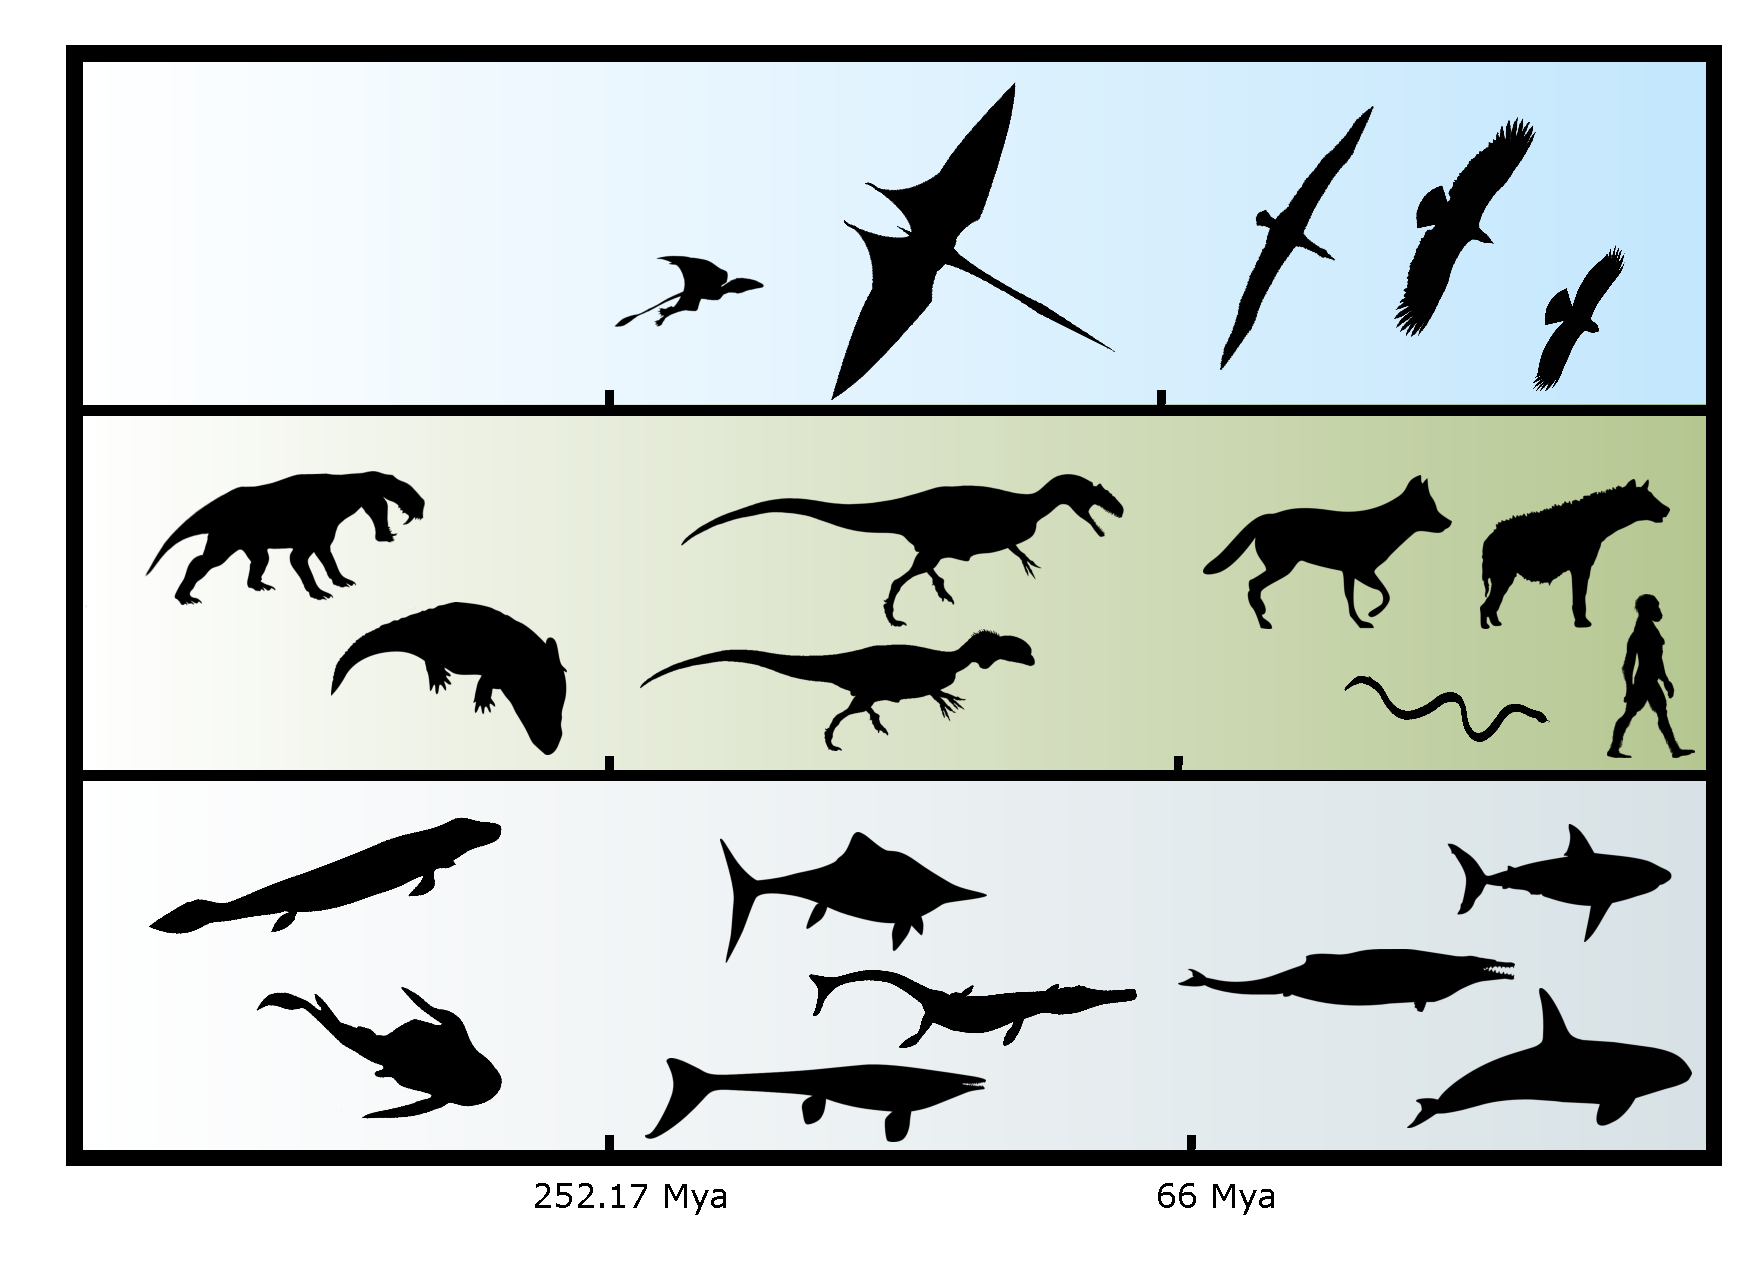
\includegraphics[width=1\textwidth]{timeline_figure/timeLine.pdf}
\caption{The diversity of scavengers through time. Each species has either direct evidence for it being a scavenger or would be positioned high up on our scavenging scale.}
\label{Timeline}
\end{figure}


\section*{Conclusion} 
As is often the case in science, the present provides the key to the past.
The animals of today, while often different (sometimes radically so) to their ancestors, can be used to make informed comparisons to extinct species. 
We have used this technique to give insight into the drivers of scavenging across vertebrates through time.
In common with any other forager be they grazer, browser or predator, scavengers past and present have had to balance their energetic costs with the gains of food. 
The main factors we considered namely, encounter rate, handling time and prey availability can be used to create a scale of scavenging whereupon any species can be placed in order to establish the importance of carrion in it diet.
We hope this approach will be useful in the effort to explore this most understudied of feeding ecologies. 
% Add bits on climate change/dectection rate change, etc...

\section*{Appendix}
Scaling relationships for sustainable travel speed are 1.15 $\times$ body mass (kg) \textsuperscript{0.12} and 0.23 $\times$ body mass (kg) \textsuperscript{0.12} for mammals and reptiles respectively \citep{ruxton2004obligate}.
These are fed into the foraging model $\sfrac{\frac{\text{duration} \times \text{speed}}{2}}{1000}$ \citep{Enstipp2006Energetics}.

\section*{Acknowledgments}

A lot of people are to thank here.


\newpage


\bibliography{bibfile}



\end{document}





%TG: what do you mean by their position? Phylogenetic? Position on the "scavenging scale"?


% This point illustrates how the environment can impact search efficiency depending on the sensory system that's used.






 


 


% \section*{Terrestrial Scavengers}

%\cite{ruxton2004obligate} offer a reason for this in that the traits that allow for vultures to exist as scavengers undermined their ability to hunt but that the same forces have not prevented mammals from doing so.


%\subsection*{Environment}




%TG: To be modified and inserted somewhere:

%TG: orginal sentence "The intertidal environment provides a ready food source of stranded marine animals on a twice-daily basis, in the immediate vicinity of the sea, and would thus have allowed marine ancestors of tetrapods gradually to acquire terrestrial competence while accessing a new and essentially untouched resource." 









 








% and sensory perception \citep{farlow1994speculations}.









 




%\section*{Aquatic Scavengers} 
%An aquatic environment presents challenges for direct observational studies and so, similar to the approaches involving extinct species, much work has approached the question of scavenging propensity from an energetics perspective.
%But it is certainly known to occur in many aquatic vertebrates.

%A point to note is that vertebrates are relatively rarer in aquatic environments, because even large animals can get support from the buoyancy of the water without needing a backbone.


%\subsection*{Locomotion}


%\subsection*{Detection}
%The existence of an obligate scavenger in a marine setting is uncertain \citep{britton1994marine,smith2003ecology,ruxton2004energetic,ruxton2005searching}.
%Depending on the species, a carcass in this environment either floats or descends to the sea floor \citep{Whitehead415}.
%In the latter low-light environment, visual detection distances are far lower (< 100 m) than they would be in the air.
%As such, animals detect resources through chemo- and mechanoreception more so than through vision \citep{ruxton2004energetic}. \cite{beasley2015vertebrates} do note that ``some benthic scavengers (e.g., hagfish: family Myxinidae) rely on necrophagy for a large portion of their diet and may indeed be obligate scavengers".




%\subsection*{Processing}


%\subsection*{Environment}

%Primary productivity is lower in almost all aquatic systems than terrestrial systems (except deserts) so as we go up the food chain the density of carcasses worth scavenging is going to be lower.










% Maybe drop this bit
% \section*{Ecological Role}
% It is recognised that scavengers keep energy flows at a higher trophic level in food webs than decomposers because they consume relatively more carrion \citep{devault2003scavenging}.
%They are also hugely important for the dispersal of nutrients \citep{beasley2015vertebrates}.
%Consider the diversity of animals that can end up feeding at the carcass of an elephant.
%Here we have an incredibly dense and nutrient rich patch that ends up being distributed widely.
%In the absence of vertebrate scavengers, invertebrates and microorganisms would consume the carcass in-situ or at least distribute the constituent nutrients over a much shorter range.
%This effect has been magnified as vertebrates evolved certain key traits that allowed them to range farther, namely an upright gait, an endothermic metabolism and of course, flight.
%To quantify this effect with a simple example we can turn to some allometric relationships relating sustainable travelling speed to body mass.
%In the case of mammals and reptiles these are 1.15 * body mass (kg) \textsuperscript{0.12} and 0.23 * body mass (kg) \textsuperscript{0.12}
% respectively \citep{ruxton2004obligate}.
%We can insert these into a foraging radius model ((duration * speed)/2)/1000 for a 12 hour foraging day which shows that while a 10 kg reptile can range 6.5 km an equally sized mammal can range nearly 33 km \citep{Enstipp2006Energetics}.
%Thus, in an ecological context, the evolution of these steps coupled with the ability to scavenge resulted in a world with a far more widely distributed nutrient landscape.





% %TG: LaTeX format template for the equations in the R file
% \begin{equation}
%   \text{Travelling speed} = \frac{duration \times speed}{2} \times 10^3
% \end{equation}
% where \textit{C} is a constant of $1.15$ for mammals and $0.23$ for squamates, %TG: if you meant squamates from reptiles
% and speed being:
% \begin{equation}
%   speed = C \times M^{0.12}
% \end{equation}


 
%Scavenging is a widespread behaviour among vertebrates where most if not all carnivores act as facultative scavengers.
%TG: or something more along the lines as:
%Most if not all carnivorous vertebrates are facultative scavenging behaviour to some extant.
%It is recognised that scavengers have an important role in keeping energy flows at a higher trophic level in food webs than decomposers because they consume relatively more carrion \citep{devault2003scavenging}. 
%Scavengers also provide useful ecosystem services by acting as barriers to the spread of disease by quickly consuming rotting carcasses which have often died from illness \citep{ogada2012dropping}.
%(Since we are intrested in scavanging in th paleo record ecosystem services might not be that relavent, although modulators of disease is still relavent) 





%The limitations in studying extant scavenging behaviour is much larger in extinct species and systems with the obvious lack of observational data available.
%TG: or more like this? 
% The limitations in studying scavenging in extant species are even bigger in extinct species and past systems since the obvious lack of available direct behavioural data (CITE) %TG: bet you there's some paper for that
% This means indirect observations in the fossil record and other approaches such as energetics must be used to infer these behaviours. %TG: I'll squiz your Am Nat paper here!
% One avenue to infer scavenging from palaeontological data can be achieved by determining if a prey item was simply too big for the carnivore to have tackled in cases where tooth marks are found \citep{pobiner2008paleoecological}. 
% Comparative analysis can also allow us to ascertain which morphologies and physiologies are likely to have been found in scavenging species in the past \citep{ruxton2004obligate}.
% The development of indirect measures of scavenging in palaeontology can in turn be applied to current scavenging systems that also suffer from a lack of observational data.

%§4
% In this review we collate methods (could this be another way of structuring it, just an idea) and research form palaeontology relating to scavenging behaviour and show that ignore this literature would be a missed opportunity for understanding extant scavenging.
%TG: totally agree. I think we need to clearly know what this review is about: scavenging through time (like a story line of scavenging past and present - a bit boring if I can speak my mind) or how to study scavenging (through time or any other aspect - probably more interesting to more people I guess).
%TG: additionally I find the divisions land/air/sea and Ceno/Meso/Paleozoic are a bit scholar. It might be better to just discuss the different techniques for investigating scavenging and include land/air/sea and Ceno/Meso/Paleo in there no? For example:
%\section{Method 1: direct observation}
%This can be totally doable in extant system for scavengers everywhere.
%It is advantageous because it's direct and reliable observations.
%But it has some limitations such as sending Adam to sit in the sun for ours and is hard to apply in deep sea environements or in any past ecosystems...



%remember the journal is an ecological one at heart so I would always keep in mind about making it useful for ecologists over paelo people. In particular from the website "ECOGRAPHY publishes papers focused on broad spatial and temporal patterns, particularly studies of population and community ecology, macroecology, biogeography, and ecological conservation. Studies in ecological genetics and historical ecology are welcomed in the context of explaining contemporary ecological patterns".



%"However, in general, vertebrate scavenging represents the widest dispersal of nutrients and energy from carcasses as vertebrate movement scales away to the broader landscape" \citep{benbow2015introduction}

 %"Increased kill rates by top predators may represent a little acknowledged marginal cost to the vertebrate community, directly attributable to scavenging activity. Given the impor -tance of top-down effects in many ecosystems, even a minor alteration to predation rates as driven by vertebrate scavengers may cause a significant flux in community composition."\citep{benbow2015introduction}

 %"Cortés-Avizanda et al. (2009) found that the abundance of prey species (i.e., hares—Lepus spp. and squirrels—Sciurus spp. in this case) decreased in sectors containing a carcass based on evidence from tracks in snow. An interesting hypothesis emerged, in which the scavengers that are recruited to a carcass may have temporarily played the dual role of increasing predator abundance near each carcass"\citep{benbow2015introduction}


%"Historically, the prevalence of scavenging activities has been greatly underestimated. However, upon recognition that (1) in most ecosystems, a large number of animals die from causes other than predation and thus become available to scavengers; (2) most carcasses are scavenged by vertebrates before they are completely decomposed by arthropods and bacteria; and (3) almost all carnivorous animals are facultative scavengers, the importance of scavenging in food webs seems unsurprising" \citep{benbow2015introduction}

%"This dispersion of carrion biomass by vertebrates is especially evident when carrion is initially concentrated spatially. For example, carcasses produced from fishing by-catch (Furness 2003), salmon (Salmonidae) die-offs (Hewson 1995), forest fires (Blanchard and Knight 1990), and single large carcasses (e.g., whales—Cetacea; Smith and Baco 2003) are often visited by multiple scavengers that range widely and therefore transport the nutrients from those carcasses over large distances."\citep{benbow2015introduction}

%"Cross-habitat nutrient transport can produce a variety of important outcomes in recipient systems (e.g., Polis et al. 2004), and scavengers can play a significant role in moving ``ecologi -cal subsidies" between habitats. For example, the use of ocean-derived carrion by terrestrial mammals (Rose and Polis 1998) and birds (Schlacher et al. 2013) is extensive and may strongly influence dynamics of coastal food webs."\citep{benbow2015introduction}

% "Markandya et al. (2008) estimated that the total costs to human health (including rabies cases from dog bites) that resulted from severe vulture declines totaled over $34 billion from 1993 to 2006. Also, Ogada et al. (2012) determined that the exclusion of vultures from large animal carcasses in Kenya resulted in a tripling of carcass decomposition times."\citep{benbow2015introduction}

%"Of all the mammalian carnivores in Africa, brown, striped, and spotted hyenas (hereafter referred to simply as hyenas) derive the largest portion of their diet from scavenging. This is not surprising, as they show many unique adaptations specifically for scavenging. They have a unique body posture and a ``rocking-horse" gait (Eloff 1964; Tilson and Henschel 1986; Hofer and East 1993a; Frank 1996) that allows them to cover long distances in search of carrion and prey."\citep{benbow2015introduction}



%\textit{Allosaurus} tooth marks on a hadrosaur in the Late Jurassic. 
% Late Triassic scavenging on a prosauropod by basal carnivorous archosaurs \citep{hungerbuhler1998taphonomy}.
%A likely instance of scavenging between a 4-million-year-old white shark (\textit{Carcharodon}) and mysticete whale from Peru \citep{ehret2009caught}.
%Bite marks on early Holocene Tursiops truncatus fossils from the North Sea indicate scavenging by rays (Chondrichthyes, Rajidae) \citep{van2009bite}. 
%Possible scavenging on a juvenile fur seal from the Late Neogene \citep{boessenecker2011mammalian}. 







